\documentclass[class=article, crop=false]{standalone}
\usepackage[utf8]{inputenc}
\usepackage{graphicx}
\renewcommand{\baselinestretch}{1.5} 
\usepackage{wrapfig}
\usepackage{subcaption}
\usepackage{caption}
\usepackage{float}
\usepackage{xcolor}
\usepackage{amsmath}
\usepackage{blindtext}
\usepackage{import}
\usepackage[backend=biber, style=numeric, citestyle=nature, doi=false, isbn=false, url=false, eprint=false]{biblatex} % Imports biblatex package, Comment out main doc
\addbibresource{refs.bib} %Import the bibliography file, Comment out main doc

\begin{document} 
\label{section:Glucose}

\section{Introduction}

Deuterium metabolic imaging (DMI) is a magnetic resonance spectroscopic imaging (MRSI) method that enables substrates and metabolic products that are labelled with the non-radioactive hydrogen isotope, deuterium ($^2$H), to be mapped in vivo. The scientific impact of $^2$H and usage in the real world has increased greatly since its existence was first theorised\cite{Urey1932AConcentration}, and it was not long before its potential for biological applications was recognised\cite{Schoenheimer1935DeuteriumMetabolism, Schoenheimer1938TheMetabolism}. Of particular interest is the use of glucose as the administered labelled precursor molecule, which can provide a direct probe of glucose metabolism. Whilst the most common current uses for $^2$H in vivo involves deuterated glucose, initially it was D$_2$O that was ingested to elevate $^2$H levels for use in nuclear magnetic spectroscopy (NMR)\cite{Brereton1986PreliminarySpectroscopy, Irving1987InSpectroscopy}, to look at lipid metabolism. The most useful forms of deuterated glucose are those whose carbon-bonded hydrogen atoms in the first and sixth positions have been replaced by deuterium because these substitutions are the only ones that are transferred to pyruvate, and then to either lactate (Lac) or to a combination of glutamate and glutamine (Glx) via the tricarboxylic acid (TCA) cycle in the mitochondria. For this reason, [6,6'-$^2$H$_2$] glucose has been a common choice of labelling (isotopologue), providing twice the number of deuterium labels as would [1-$^2$H] glucose, and has been used in many \textit{in vivo} studies from preclinical work\cite{Lu2017QuantitativeSpectroscopy, Meerwaldt2023InImaging} to the demonstration in humans\cite{DeFeyter2018DeuteriumVivo, Roig2022Deuterium7T}. Lactate and Glx as well as non-metabolised glucose and water (natural abundance plus an additional amount caused by label-loss during various processes) become detectable via either choice of labelling. The detected lactate and Glx provides information about the cell’s propensity to metabolise glucose via glycolysis or the oxidative phosphorylation pathway, and thereby an important clinical potential of DMI is identified since many tumour cells exhibit an increased tendency for glycolysis, which manifests in higher than usual lactate production;  the well-known Warburg effect\cite{Warburg1956OnCells}.    

This technique allows information on downstream metabolite concentrations to be quantified as well as tracked to obtain metabolic flux measurements, without the use of ionising radiation in a similar way to what is most commonly used positron emission tomography (PET) scans. Besides tumours and other disease states, brain metabolism may also be altered, albeit temporarily, as part of its normal functioning. This might occur when a part of the brain is activated by a task or stimulus, such as by visual stimulation. It has been previously shown that there is metabolic activation in the visual cortex following visual stimulation\cite{Kushner1988CerebralStimulation, Beland-Millar2018FluctuationsStimulation}. Consistently using $^1$H lactate increases\cite{Prichard1991LactateStimulation., Sappey-Marinier1992EffectSpectroscopy, Fernandes2020MeasurementT}, and glucose decreases\cite{Lin2012InvestigatingT} in the visual cortex following visual stimulation has been measured. and $^{13}$C\cite{Chhina2001MeasurementSpectroscopy} MRS, $^{31}$P has also been used to measure metabolism changes\cite{Sappey-Marinier1992EffectSpectroscopy} however glucose and lactate signals are not present here. It is important to note that significant increases in glutamate and decreases in glutamine have also been shown\cite{Lin2012InvestigatingT}, since Glx is the combination of the two metabolites a statistical change in Glx is unlikely. 
 
In its simplest implementation of spectroscopic imaging, DMI is relatively straightforward to set up with a pulse-acquire chemical shift imaging (CSI) sequence, usually without the need for water suppression because of the low concentration of naturally occurring deuterated water. In most cases, the DMI spectra are also simpler to analyse than the proton spectra. If using glucose as the labelled substrate, there are just four metabolites to consider: water (HDO), glucose, Glx, and lactate. This relative simplicity can be regarded as a positive attribute in the context of potential clinical translation. However, the generally low SNR of DMI is not a favourable characteristic, and means that data is often acquired with low spatial resolution often around 8 ml\cite{DeFeyter2021DeuteriumFuture, deGraaf2020OnImaging} in volume, with the smallest to date being reported in humans is 2.97 ml\cite{Ruhm2022Dynamic9.4T}, at a high magnetic field strength of 9.4 T. Low SNR and spatial resolution can potentially be improved upon by performing DMI scans through indirect detection using $^1$H MRSI\cite{vanZijl2020SpectroscopicFluxes, Bednarik2021DeuteriumBrain, Niess2023Reproducibility3T, Ruhm2022Dynamic9.4T}, with the additional benefit of not requiring deuterium-specific hardware, but at expense of often requiring a more complex acquisition scheme and post-processing analysis. Another method of increasing SNR in DMI is to implement de-noising during post-processing analysis, this has been shown to improve SNR in MRSI using low rank approximations\cite{Nguyen2013DenoisingApproximations}. Similar techniques using Tucker decomposition\cite{Tucker1966SomeAnalysis, Bader2007EfficientTensors} have been applied to DMI MRSI data with notable SNR improvements\cite{vonMorze2021ComparisonT, Kreis2020MeasuringMRI}.

More than just D$_2$-glucose has been used to investigate in vivo metabolism, [6,6'-$^2$H$_2$] fructose has been used to investigate liver cancer\cite{Zhang202366-2H2Cancer}. Fructose was found to have a similar spectral appearance as the glucose, with slightly different kinetics. After deuterated acetate ([$^2$H$_3$] acetate) is intravenously injected it has been used to investigate myocardial metabolism\cite{Wang2021NoninvasiveImaging} and tumour metabolism\cite{DeFeyter2018DeuteriumVivo}, where acetate accumulation and glx changes are tracked. One approach to increasing the deuterium signal is to use a form of deuterated glucose with a larger number of deuterium labels. Since there are twelve hydrogen atoms in the glucose molecule, all twelve could be substituted with deuterium atoms. However, those in the hydroxyl groups tend to exchange rapidly with the surrounding water and therefore are not usually useful in metabolic applications. However, the seven locations in which the deuterium atoms are directly carbon-bonded are less labile and potentially useful, yielding the form [1,2,3,4,5,6,6'-$^2$H$_7$]glucose (D$_7$-glucose). Compared with [6,6'-$^2$H$_2$]glucose (D$_2$-glucose), the deuterium spectrum would contain a factor of 7/2 more components, many of which would overlap due to the broad linewidths, producing a gain in SNR. The deuterium atoms in the C1 and C6 positions (in the absence of label-loss) will be transferred to lactate or Glx molecules\cite{DeFeyter2020DeuteriumBrain}, producing a gain of 3/2. Therefore, it is expected that the use of D$_7$-glucose will increase the SNR and reliability of detected signals for glucose, Glx, and lactate, compared to using D$_2$-glucose. In addition, the four remaining deuterium labels in the positions C2 – C5 of D$_7$-glucose are transferred directly or indirectly to water during glycolysis, and will therefore contribute to an increased HDO signal\cite{Mahar2020HDOMetabolism, Mahar2021DeuteratedGlucose}. The HDO (deuterated water) signal increase that is a result from metabolism has been shown to be directly proportional to the increase in downstream metabolites (glx and lactate)\cite{Mahar2021DeuteratedGlucose}, which implies that regular non-spectroscopic imaging of the HDO signal increase can be used as a measure of the Warburg effect with improved spatiotemporal resolution compared to MRSI/CSI techniques. 

The primary aim of this study is to measure the difference in vivo metabolite signal/concentration changes for HDO, glucose, Glx and lactate in the brains of healthy human participants following ingestion of D$_2$-glucose or D$_7$-glucose. CSI scanning, de-noising and a sophisticated and robust fitting routine is used to track the change in metabolite signals. Metabolite signals for each metabolite was found to be larger for all metabolites after ingestion of D$_7$-glucose, concentration values were also found to be larger in each metabolite except glucose. This shows that Warburg maps with better SNR can be obtained following ingestion of D$_7$-glucose that would imply a better CNR between healthy and diseased tissue in patients with brain tissues. Secondarily, the possibility of detecting differences in metabolite concentrations due to an applied visual stimulus was investigated.  

\section{Methodology}

\subsection{Particicpants}

Scanning was performed on a 7T Achieva scanner (Philips Healthcare), operating at 45.8 MHz for $^2$H. A 26.4 cm inner-diameter, dual-tuned $^1$H/$^2$H birdcage RF coil (Rapid Biomedical) was used for deuterium measurements and anatomical $^1$H images. Ethical approval was received from the Faculty of Medicine and Health Sciences Research Ethics Committee (ref. no. FMHS 306-0621) at the University of Nottingham to recruit 15 healthy participants for this study. Informed consent was received from all participants and recruited if they had a BMI $<$ 25 kg/m$^2$ (or less than 27 kg/m$^2$ for males if their waist circumference was $<$94 cm), had a normal heart rate and blood pressure, a blood glucose concentration of $<$7.8 mM (finger-prick test), were between 18 and 60 years old, and had no significant medical conditions or issues related to safety in the MR scanner. At the screening visit, participants were informed whether visual stimulation would be applied and that at least an eight hour fast is required on the day of scanning, this was checked using a second blood glucose level test (finger-prick) that had to be $<$5.6 mM. For those receiving D$_2$-glucose (n=8), 5 experienced a visual stimulus. For those receiving D$_7$-glucose (n=7), 4 experienced a visual stimulus.

\subsection{Scan Protocol}

Scanning for each participant was split into two parts, the baseline natural abundance scans before the glucose drink which are used for quantification and calibration lasting approximately 20 minutes, and the 90-minute scan session after the glucose drink was ingested. The drink was consumed in a maximum of eight minutes. Baseline measurements included a $^1$H scout scan for planning; a $^1$H MPRAGE scan (FOV = 224 x 224 x 140 mm$^3$, 1.4 mm isotropic voxels, TR = 7.1 ms, TE = 2.6 ms, with a scan duration of 353 s); a non-localised $^2$H spectrum (16 averages, TR = 1000 ms, TE = 1.1 ms, flip angle = 90$^\circ$, bandwidth = 3000 Hz, 2048 samples, with a scan duration of 17 s); a slice-selective $^2$H spectra were acquired from a 2-cm-thick axial slice positioned over the lateral ventricles, using 128 averages, TR = 1000 ms, TE = 1.9 ms, flip angle = 90$^\circ$, bandwidth = 3000 Hz,  2048 samples, having a scan duration of 129 s and a 3D $^2$H chemical shift image (CSI) covering the whole brain (FOV = 180 x 180 x 120 mm$^3$ , 15 mm isotropic voxels, TR = 230 ms, TE = 2.4 ms, flip angle = 62$^\circ$, bandwidth = 1200 Hz, 256 samples, with a scan duration of 670 s) acquired using 6 acquisition-weighted\cite{Pohmann2001AccurateCSI} averages. All the natural abundance scans were performed in the absence of visual stimulation. The participant was then brought out of the scanner and consumed the glucose drink, this contained 0.75g/kg (bodyweight) of either D$_2$ or D$_7$-glucose powder—purchased from CK Isotopes Ltd. (microbiological/pyrogen-tested product) and Merck Life Science UK Ltd. (endotoxin-tested product)—dissolved in 250 ml of water at room temperature. The participant was allowed to consume this in their own time, and when they indicated that they were ready for the second scanning session (<30 minutes later), were guided back into the scanner.

% Scan detail table instead of it included in text

In the second session, the two $^1$H scans were repeated, followed by five or six repeats of the three $^2$H scans. In the event that the participant needed to exit the scanner for a short period and re-enter, the $^1$H scans were repeated before continuing with the deuterium scans. If the participant was to be visually stimulated, the display would be activated during the CSI scans only and quiescent otherwise.  

Visual stimulation was achieved via an 8 Hz flashing, black and white, radial checkerboard, similar to what has been used previously\cite{Fernandes2020MeasurementT}. The visual display was projected onto a screen that the participants could observe while lying in the scanner by wearing prism glasses. Most of the participants who experienced visual stimulation (three that ingested D$_2$-glucose and four that ingested D$_7$-glucose) experienced a checkerboard flashing pattern that was active for 50 seconds followed by 10 seconds of a red cross on a grey background. However, two participants (both of whom ingested D$_2$-glucose) experienced a checkerboard flashing pattern that was active for 30 seconds followed by 30 seconds of a red cross on a grey background. Participants who received no visual stimulation were asked to close their eyes. In all cases, the scanner room lights were turned off. 

% Scan Protocol image

\subsection{Image and spectral processing}

The $^1$H MPRAGE image was converted to a NIFTI format using MRIcroGL (www.nitrc.org), and bias-field corrected using FSL-FAST\cite{Zhang2001SegmentationAlgorithm}. The corrected MPRAGE image was then brain extracted using FSL-BET\cite{Smith2002FastExtraction} with a robust centre estimation and to further remove any bias and any neck voxels, the fractional intensity threshold was allowed to vary between subjects along with the vertical gradient. The MNI-152 brain image with 2 mm isotropic voxels (distributed with FSL\cite{Smith2004AdvancesFSL}) was linearly registered to each image obtaining the affine matrix using FSL-FLIRT\cite{Jenkinson2001AImages, Jenkinson2002ImprovedImages} and twelve degrees of freedom. The MNI-152 brain image is non-linearly registered to the same image to obtain the warp-field using FSL-FNIRT\cite{AnderssonJ2008FNIRT-FMRIBsTool}, with the affine from the linear registration used as an initial guess. The warp-field is then used to non-linearly register probabilistic maps from the MNI-152 space for the frontal and occipital lobes to the MPRAGE space. Finally, FSL-FAST\cite{Zhang2001SegmentationAlgorithm} is used on the brain-extracted MPRAGE image to probabilistic maps for cerebrospinal fluid (CSF), grey matter (GM) and white matter (WM), with the affine matrix used to improve initialisation. The CSF mask was manually segmented to only include the left and right ventricles. The maps are then binarised to obtain region of interest (ROI) masks. 

In some of the CSI spectra a noise spike was visible that would affect each voxel in the same frequency position, the spike only affected one data point. To correct this the data points immediately either side of the spike were averaged together, the spike was replaced with this value. Each CSI was denoised in the time-domain using a Tucker decomposition\cite{Bader2007EfficientTensors} with a compression matrix size of [64 6 6 5] (spectral and 3 spatial dimensions), this is similar to what  matrices have previously been used with DMI\cite{vonMorze2021ComparisonT, Kreis2020MeasuringMRI} and C$^{13}$ studies\cite{Brender2019DynamicHyperpolarization}. The FID’s were fitted using an adapted version of the OXSA-AMARES MATLAB toolbox\cite{Vanhamme1997ImprovedKnowledge, Purvis2017OXSA:MATLAB}, which requires prior knowledge for each of the metabolites. The chemical shifts of glucose (both anomers), Glx, and lactate are assumed to be the same as those of the $^1$H chemical shifts\cite{Govindaraju2000ProtonMetabolites} and were implemented in the fitting as relative shifts to the water peak\cite{Meerwaldt2023InImaging}. Often in previous studies that have used D$_2$-glucose, the spectrum has been fitted as a single peak at 3.8 ppm, since the chemical shift difference between the four resonance lines (two deuterium labels, two glucose anomers) are usually not discernible due to the relatively broad linewidths and low SNR. However, this is not the case for D$_7$-glucose\cite{Govindaraju2000ProtonMetabolites} which has a larger number of spectral lines and range of chemical shifts. Therefore, the spectrum needs to be accounted for more accurately, taking into account the contribution from each deuterium label for both anomers and, for consistency, this approach has also been implemented when analysing the data after D$_2$-glucose. The glucose peaks were fitted assuming a common scaling factor; all glucose peaks have the same phase other than the peaks from the C1 position which have a different phase due to large differences in chemical shift. The linewidths of peaks from the same anomer share the same value. For HDO, Glx, and lactate, only single components were assumed, with independent amplitudes, phases, and linewidths.

The amplitude and phase of each metabolite peak at each voxel position were converted to complex amplitudes and interpolated to the same resolution as the MPRAGE image. These maps were then averaged over the whole-brain, occipital lobe, frontal lobe, CSF, GM, and WM ROIs (using the binarised segmentation maps) to obtain ROI-averaged amplitudes for each metabolite for each CSI, which provided amplitudes as a function of time relative to glucose ingestion. These values were then either quantified into concentration values, normalised or corrected for their T$_1$ variation and used as ratios between the two different types of glucose.

% Canva/Biorender Image

\subsection{Concentration calculations}

Concentrations $C^m$ for each metabolite m were determined using the equation

\begin{equation}
    C^m = \frac{A^m}{kE^mN^m}
    \label{eqn:Glu:Conc}
\end{equation}

where $A^m$ is the FID amplitude of the metabolite, $N^m$ is the number of effective deuterium labels per metabolite molecule, $E^m$ is the attenuation factor given by

\begin{equation}
    E^m = \frac{1-\exp(-T_R/T_1^m)}{1-\exp(-T_R/T_1^m)\cos{\theta}}
    \label{eqn:Glu:Atte}
\end{equation}

where T$_1^m$ is the longitudinal relaxation time of the metabolite, T$_R$ is the repetition time, $\theta$ is the flip angle, and where $k$ is a scaling constant. This constant, which is found to be ROI-dependent, is calculated by using the average water amplitude within a given ROI, by applying Equation \ref{eqn:Glu:Conc} with an estimate of the natural abundance concentration calculated assuming an isotopic percentage for deuterium of 0.0156\%\cite{Hagemann1970AbsoluteSMOW}, a concentration of pure water at 55.4 M, a factor of 2 because of the two hydrogen atoms in water, and an estimate of the percentage of water in the ROI. Cortical grey matter (GM) and white matter (WM) were assumed to be 84\% and 69\% water\cite{Oros-Peusquens2019AImplications}. The occipital and frontal ROIs were assumed to be comprised of 40\% GM and 60\% WM, resulting in a water content of 75\%. The whole brain ROI was assumed to be 10\% CSF, 36\% GM, 54\% WM, resulting in 77\% water.

Once $k$ was calculated for each ROI, metabolite concentrations were calculated via Equation \ref{eqn:Glu:Conc}, with knowledge of the deuterium label numbers, $N^m$.

The effective number of deuterium labels depends on whether D$_2$-glucose or D$_7$-glucose is ingested and, for Glx and lactate, label-loss. For D$_2$-glucose, we have assumed the effective number of labels for water, glucose, Glx, and lactate is 1, 2, 1.2, and 1.7, respectively\cite{DeGraaf2021CharacterizationStudies}. For D$_7$-glucose, we have assumed 1, 7, 0.9, and 1.3 (estimated\cite{Funk2017TheGlucose} assuming glutamine and glutamate are present in approximately equal amounts). 

Longitudinal relaxation times for glucose, Glx and lactate were assumed to be 67 ms, 139 ms, and 297 ms respectively\cite{DeFeyter2018DeuteriumVivo}, independent of ROI, number of deuterium labels, and of whether D$_2$-glucose or D$_7$-glucose was the metabolic precursor. For water (HDO), the T$_1$ relaxation times were 510 ms, 320 ms, and 290 ms for CSF, grey matter, and white matter, respectively\cite{Cocking2023DeuteriumDosing}. These relaxation times were used to estimate relaxation times for each ROI based on their water percentage.

\section{Results}

\begin{figure}
    \centering
    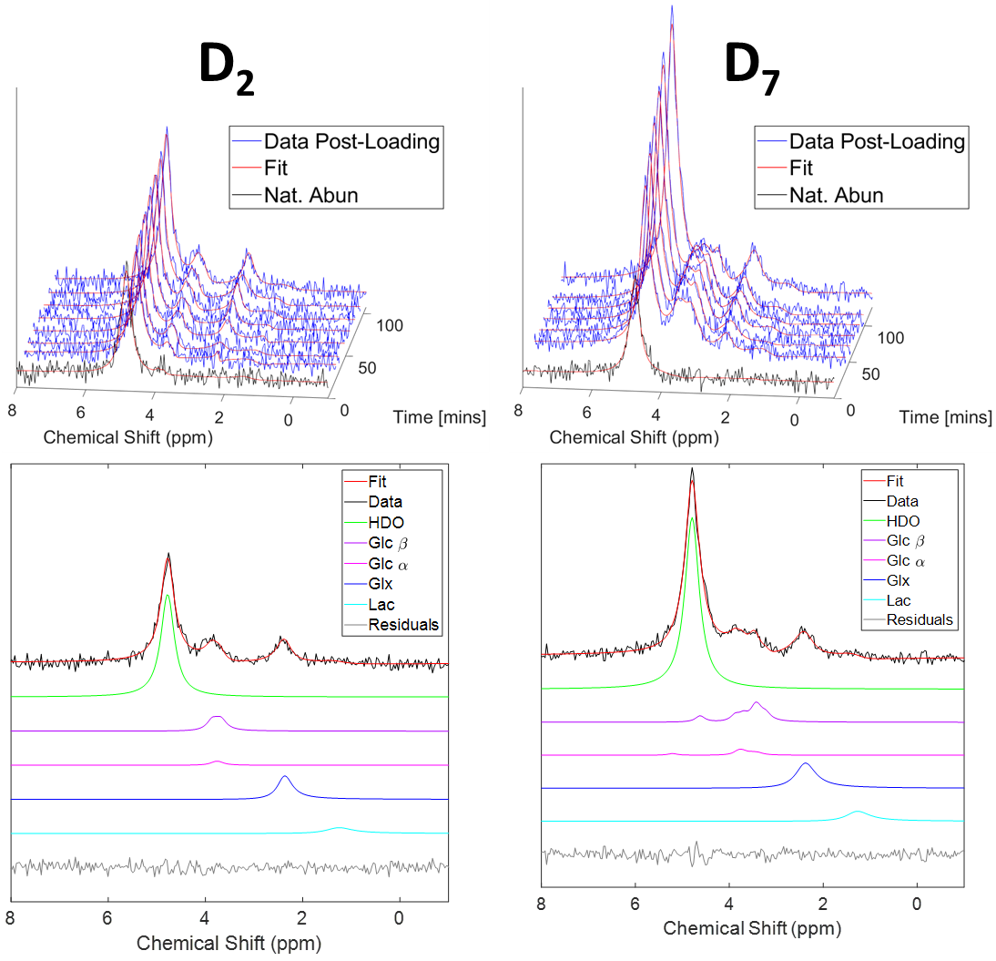
\includegraphics[width = 1\textwidth]{Figures/Glucose/Selective.png}
    \caption{Stacked selective spectra from a 2-cm-thick slice over the lateral ventricles from participants who had ingested D$_2$-glucose (a) or D$_7$-glucose (b). (c-d) Last spectra obtained during scanning with timepoints of $\approx$108 and $\approx$125 minutes respectively after glucose ingestion. Corresponding fits are shown for each spectra, along with separated contributions from each metabolite and the residuals after fitting.}
    \label{fig:Glu:Select}
\end{figure}

Figure \ref{fig:Glu:Select} shows spectra acquired from a 2-cm thick axial slice positioned over the lateral ventricles in two participants before and after ingesting D$_2$- or D$_7$-glucose. The spectra are displayed with the same signal intensity axis scale so that the greater amplitudes of the signals following D$_7$-glucose ingestion are evident, especially for the HDO. Single spectra obtained $\approx$108 minutes and $\approx$125 minutes after D$_2$-glucose and D$_7$-glucose ingestion respectively are also shown, along with the fits, and the individual contributions to the fit from HDO, glucose (each anomer), Glx and lactate. The glucose signals include contributions from each anomer ($\alpha$ and $\beta$) and each label position which is why ingesting D$_7$-glucose, centred around 3.7 ppm, produces a broader peak compared to D$_2$-glucose, with additional resonances at $\approx$5.2 and $\approx$4.6 ppm from the C1 deuterium of the two anomers. The HDO, glx and lactate signals show no obvious differences in linewidths and chemical shift position between participants (or glucose isotopologues) or times after glucose ingestion. No obvious peak is visible above the noise floor in the residual spectrum, indicating the fitting performed well, especially over the more intricate glucose signal.

\begin{figure}
    \centering
    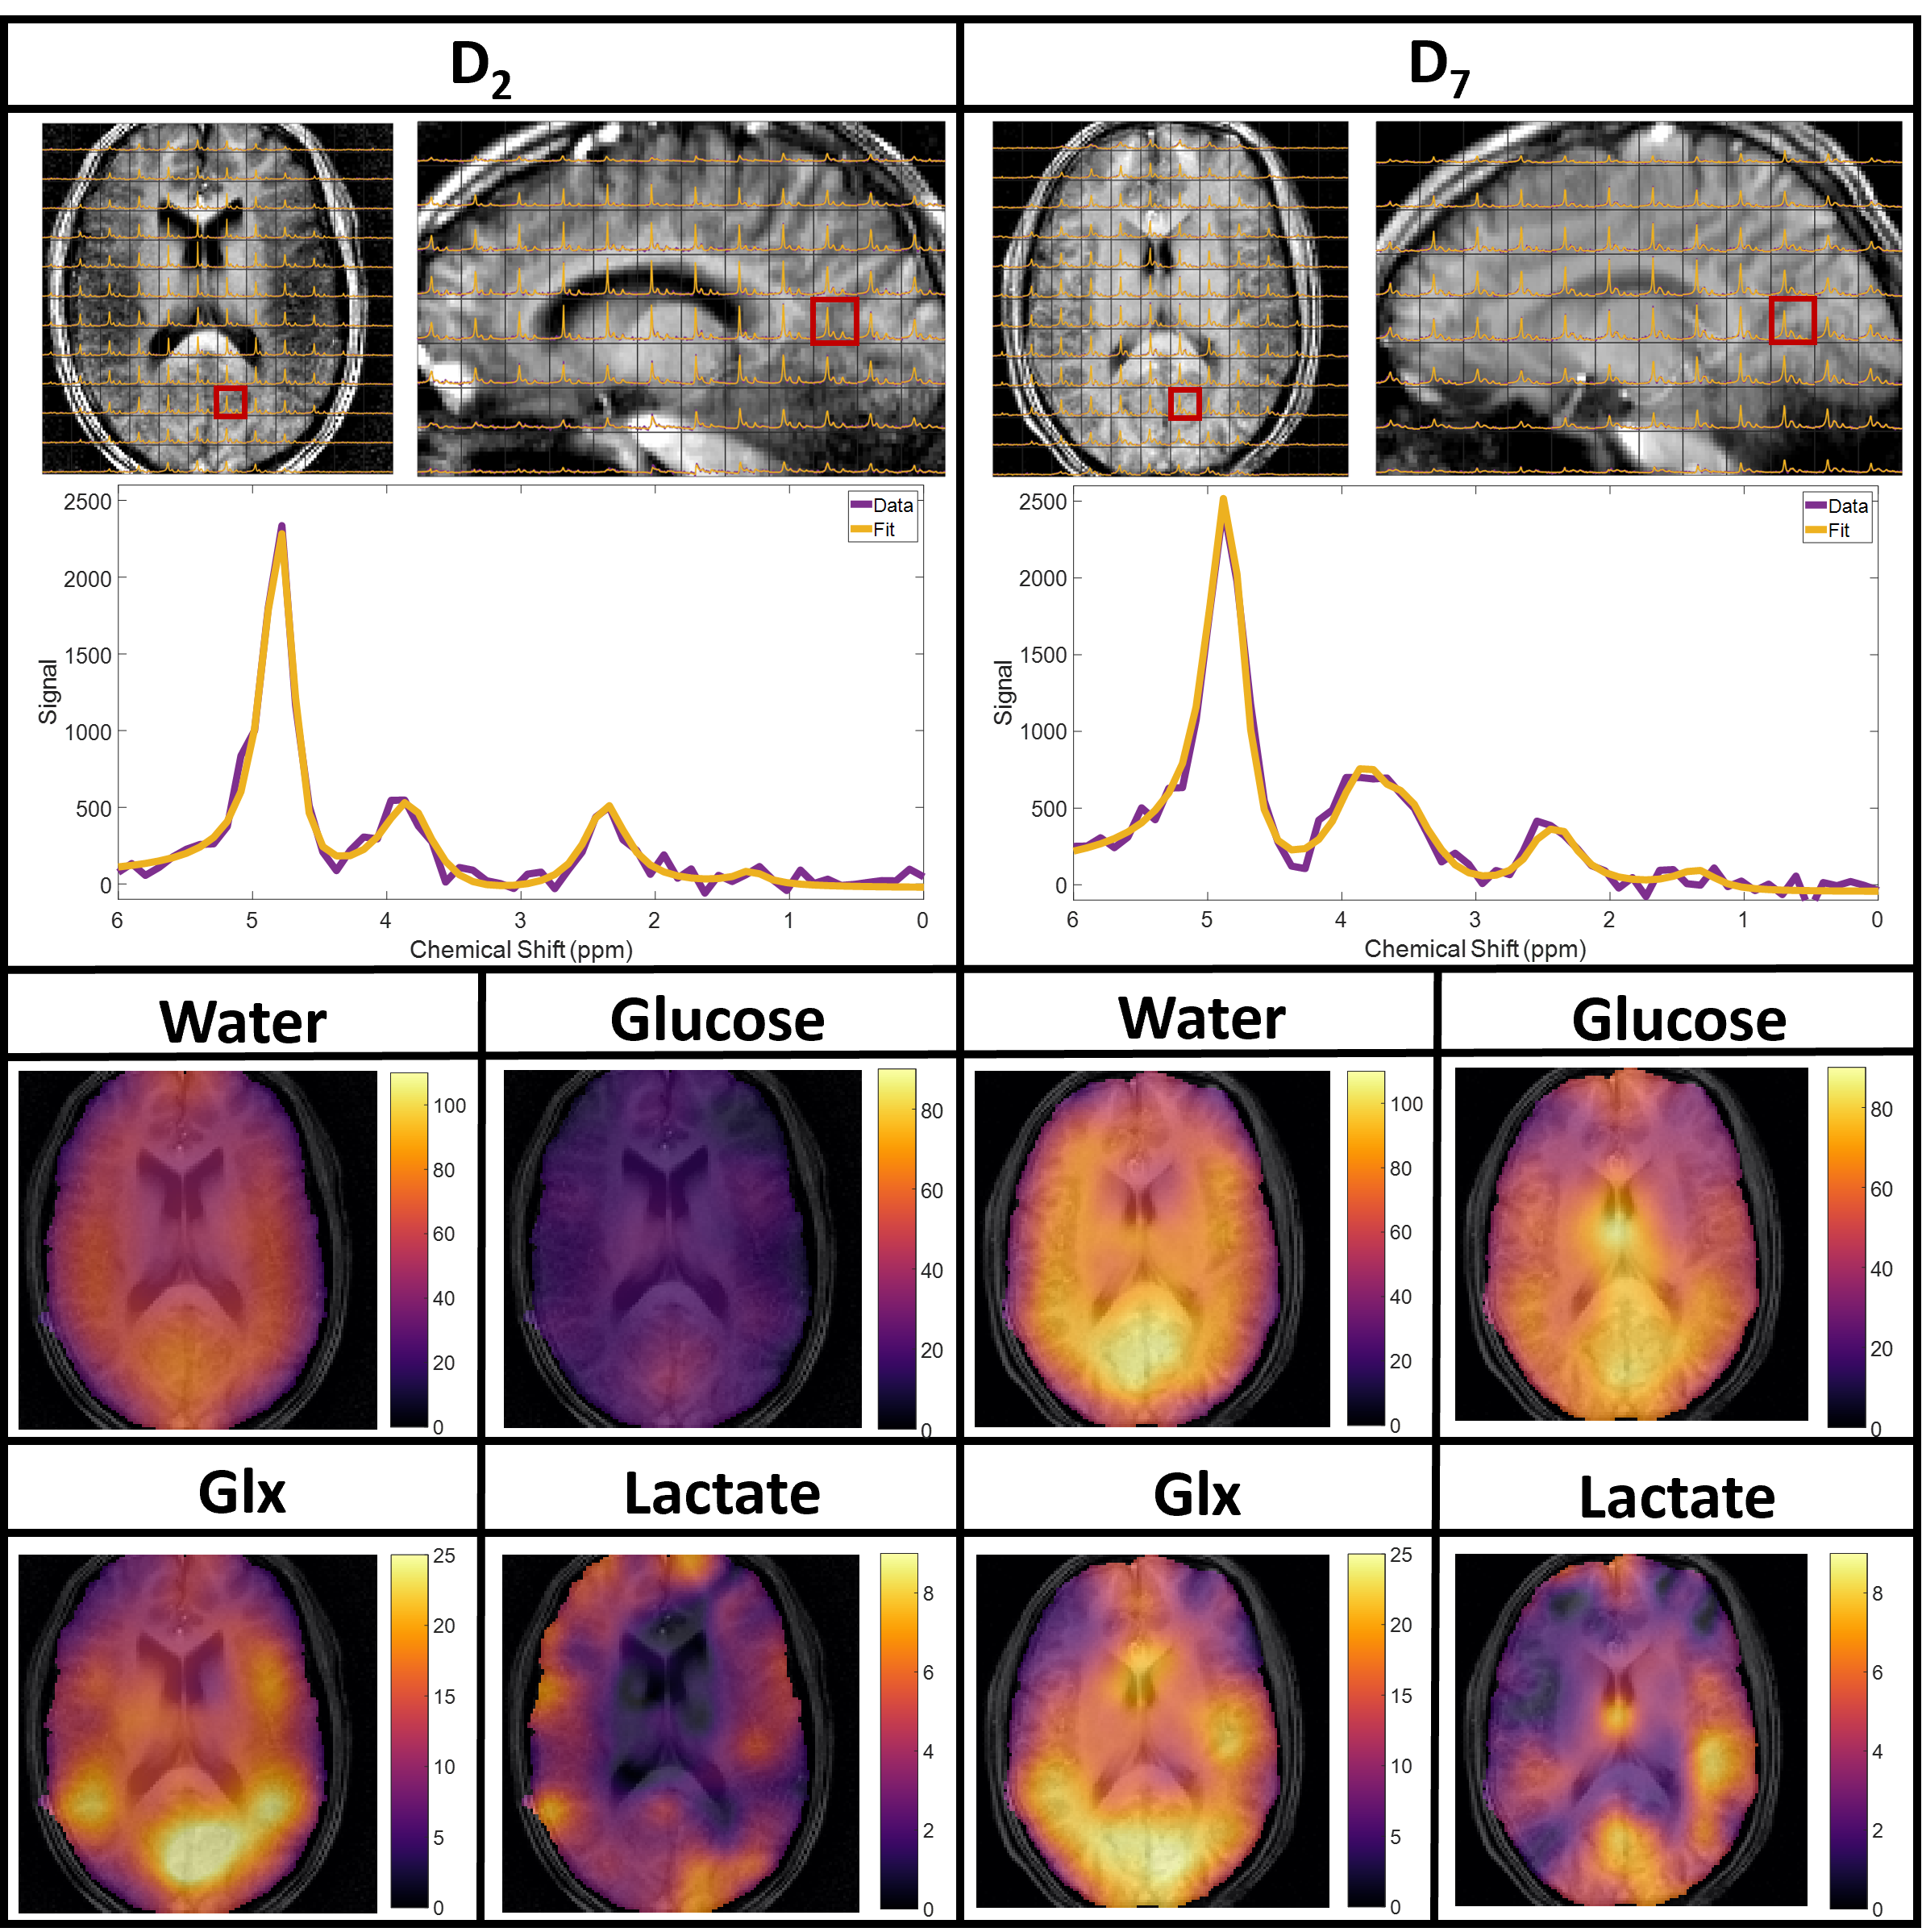
\includegraphics[width = 1\textwidth]{Figures/Glucose/CSI.png}
    \caption{Axial and sagittal slices of the 3D CSI data set (FOV = 180x180x120 mm$^3$, 15 mm isotropic resolution) from two participants each after ingestion of D$_2$-glucose (left) and D$_7$-glucose (right). Spectra were averaged over six scans and then denoised using a Tucker decomposition and are overlaid on the corresponding slice of the MPRAGE image acquired after ingestion. Experimental data (purple) and fits (yellow) are shown for each voxel. The spectra from the highlighted voxels are shown in detail in the lower plots. Amplitude maps for each metabolite are shown below, with the colour axis being shared between D$_2$-glucose and D$_7$-glucose.}
    \label{fig:Glu:CSI}
\end{figure}

Axial and sagittal slices from denoised 3D CSI data, averaged over six scans are shown in Figure \ref{fig:Glu:CSI} for two participants (D$_2$-glucose versus D$_7$-glucose), with the overall fits to each voxel, the data is overlaid on the bias-field-corrected $^1$H MPRAGE image. Spectra and corresponding fits from the highlighted voxels (red) in both the axial and sagittal view are also shown, the data appears similar in appearance to those displayed in the slice-selective spectra of Figure \ref{fig:Glu:Select}. Interpolated and overlaid, axial, amplitude maps of each of the metabolites of one slice are shown in Figure \ref{fig:Glu:CSI} after ingestion of D$_2$-glucose and D$_7$-glucose for two participants. The FID amplitude values, for each metabolite, are obtained from fitting the averaged CSI data after denoising using OXSA-AMARES\cite{Vanhamme1997ImprovedKnowledge, Purvis2017OXSA:MATLAB}.

\begin{figure}
    \centering
    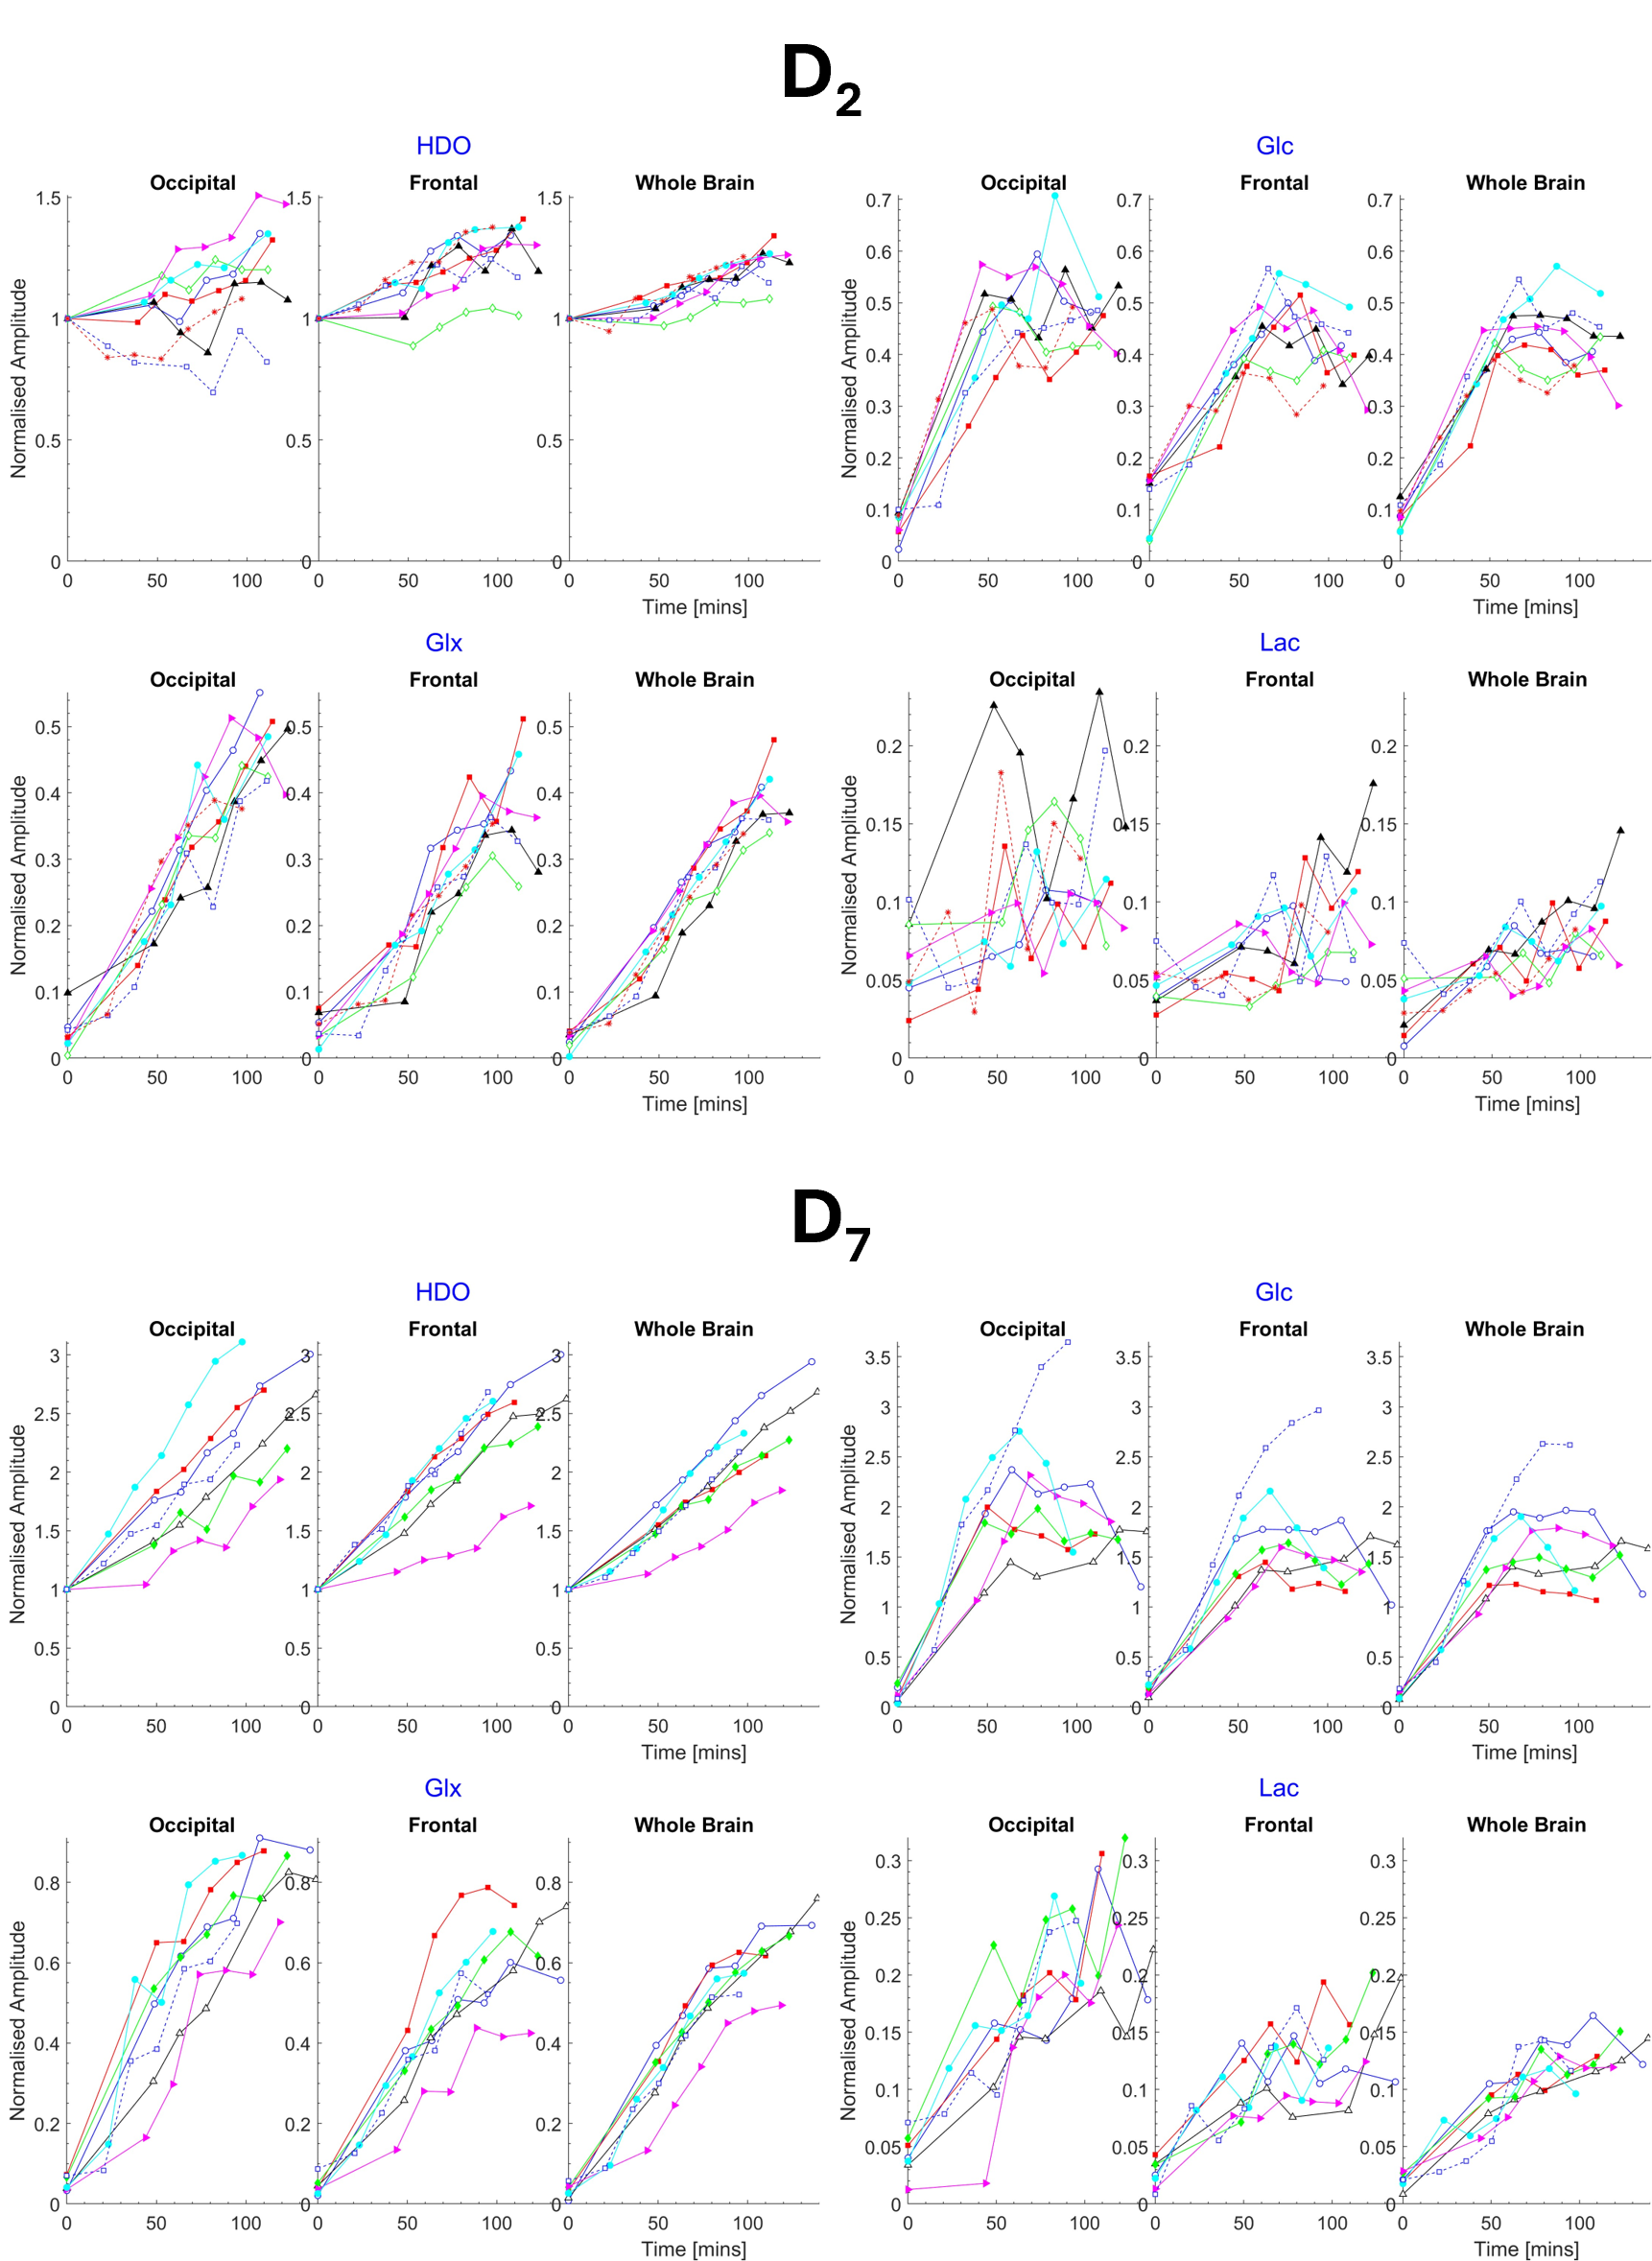
\includegraphics[width = 1\textwidth]{Figures/Glucose/Ind_Amp.png}
    \caption{Normalised metabolite signal amplitudes for each participant for D$_2$-glucose (top) and D$_7$-glucose (bottom) for each ROI: CSF, GM, WM, occipital lobe, frontal lobe, and the whole brain.}
    \label{fig:Glu:Ind_Amp}
\end{figure}

Displayed in Figure \ref{fig:Glu:Avg_Amp} are participant-averaged metabolite time-courses (non-averaged data are shown in Figure \ref{fig:Glu:Ind_Amp}). The data is created by taking a moving average of the time-ordered data from all participants in the D$_2$ or D$_7$-glucose cohorts, with a window size equal to the number of participants in that cohort. This is shown in Figure \ref{fig:Glu:Avg_Amp} with the errorbars being equal to the moving standard  amplitudes are normalised using the HDO signal at natural abundance obtained before ingestion of glucose, for each participant. The maximum in the averaged glucose signal is clearly visible and occurs between 50 and 100 minutes after glucose ingestion. In these plots, it is clear that all metabolite amplitudes from D$_7$-glucose ingestion are large than those from D$_2$-glucose. 

\begin{figure}
    \centering
    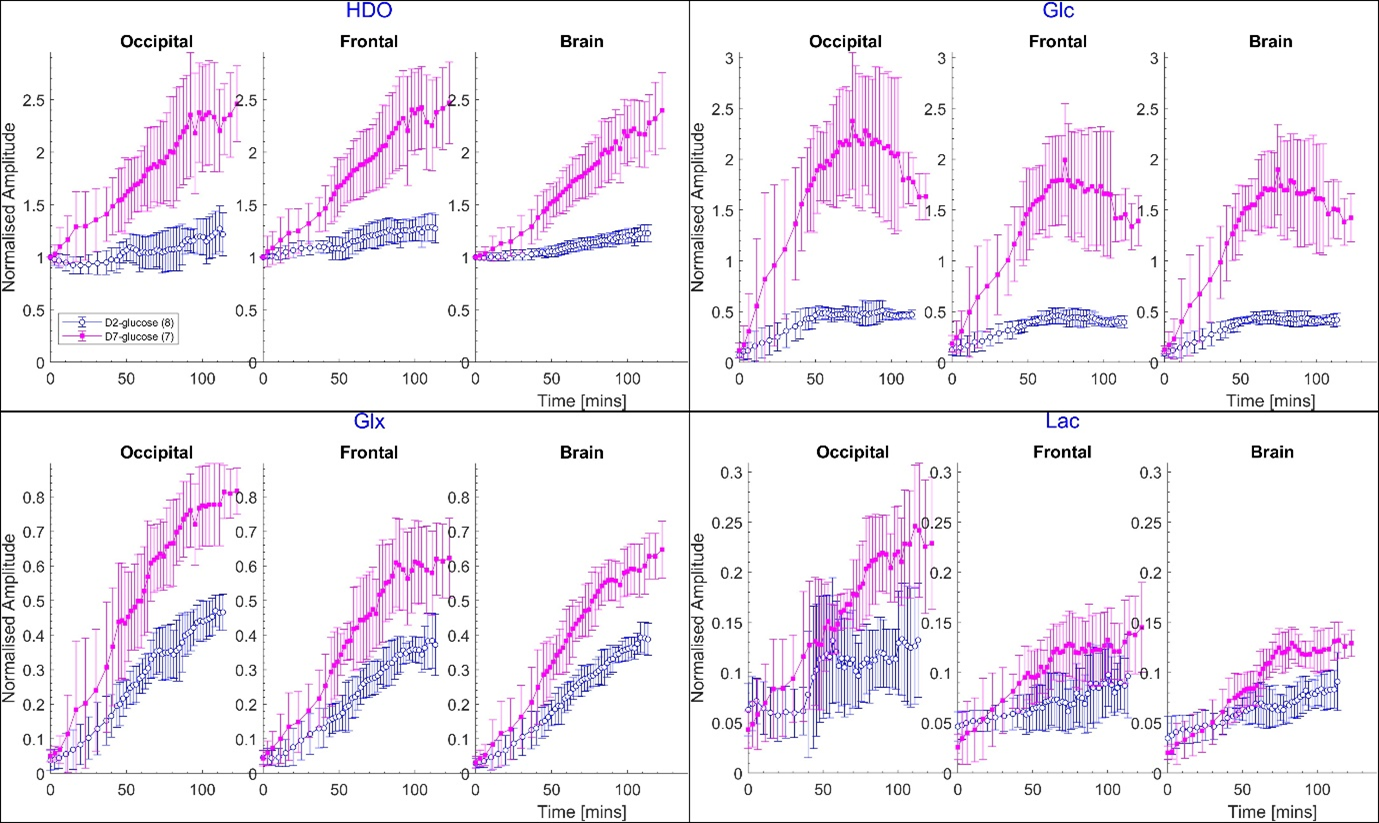
\includegraphics[width = 1\textwidth]{Figures/Glucose/Avg_Amp.png}
    \caption{Average time courses of normalised metabolite signals for CSF, GM, WM, occipital lobe, frontal lobe, and the whole brain from participants who ingested D$_2$-glucose (blue) and D$_7$-glucose (pink). A moving average which over the nearest points in time equal to the number of participants, with error bars representing the moving standard deviation.}
    \label{fig:Glu:Avg_Amp}
\end{figure}

The same data, converted to concentrations are shown in Figure \ref{eqn:Glu:Conc}. These concentrations are the corrected for label-loss, so that the values estimate the concentrations of deuterated molecules that would be observed if no label-loss occurred. As expected, the averaged concentrations of HDO, Glx, and lactate are clearly different between the D$_2$ and D$_7$-glucose cohorts, with the glucose concentrations appearing similar. 

\begin{figure}
    \centering
    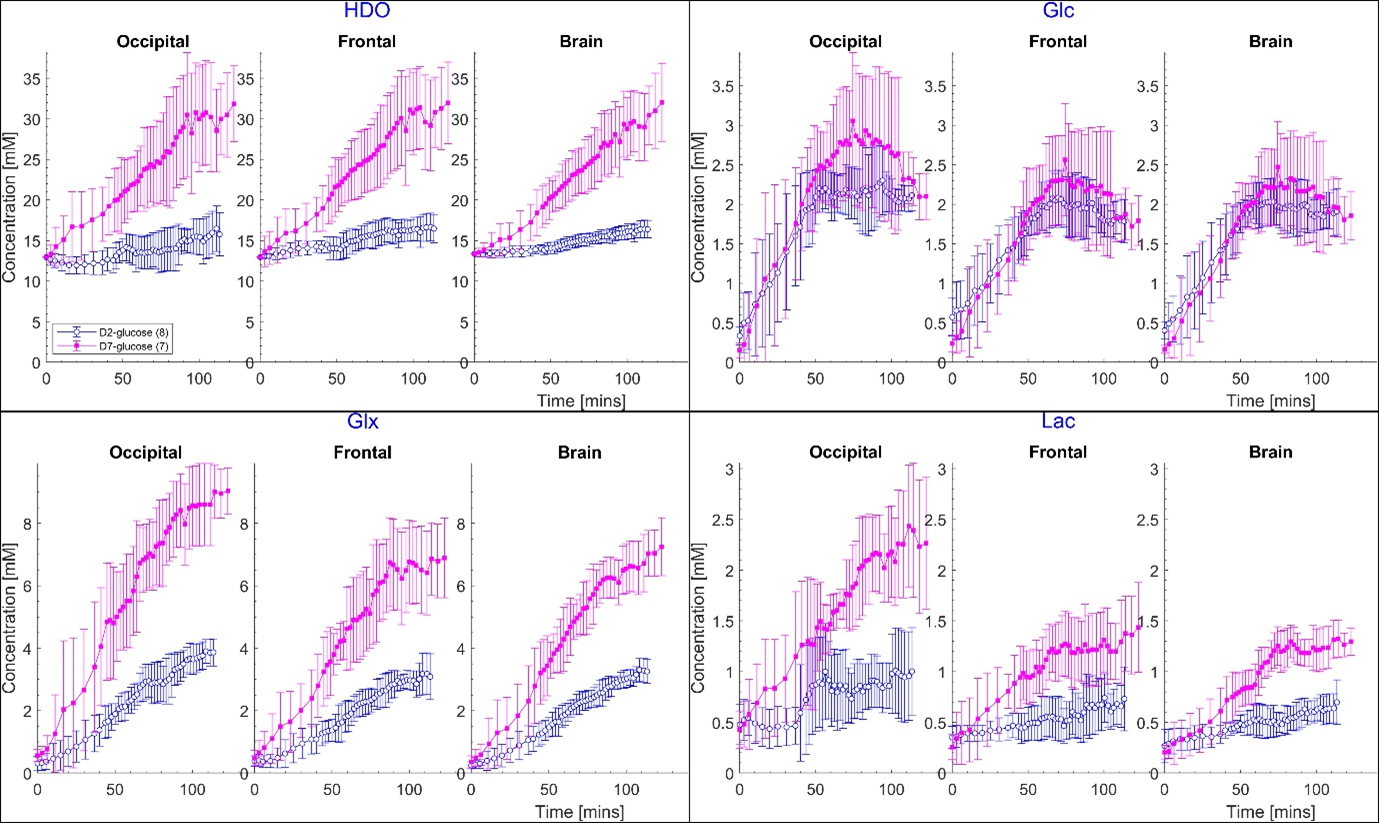
\includegraphics[width = 1\textwidth]{Figures/Glucose/Avg_Conc.png}
    \caption{Average time courses of metabolite concentrations from CSF, GM, WM, occipital lobe, frontal lobe, and the whole brain from participants who ingested D$_2$-glucose (blue) and D$_7$-glucose (pink). A moving average which over the nearest points in time equal to the number of participants, with error bars representing the moving standard deviation.}
    \label{fig:Glu:Avg_Conc}
\end{figure}

To provide a clearer depiction of the relative metabolite signal amplitudes arising from D$_2$ and D$_7$-glucose ingestion, Figure \ref{fig:Glu:D7_D2} shows plots of the ratios of metabolites from the two glucose isotopologues: Amplitude(D$_7$)/Amplitude(D$_2$). To calculate the ratio between the averaged D$_2$- and D$_7$-glucose signals, the data needs to cover the same points in time. Therefore, the D$_2$-glucose data is interpolated to the same time series data as the D$_7$-glucose data. The error bars are derived from the error bars (standard deviations) of the numerator and denominator by the standard method of combining independent errors of a quotient. 

\begin{figure}
    \centering
    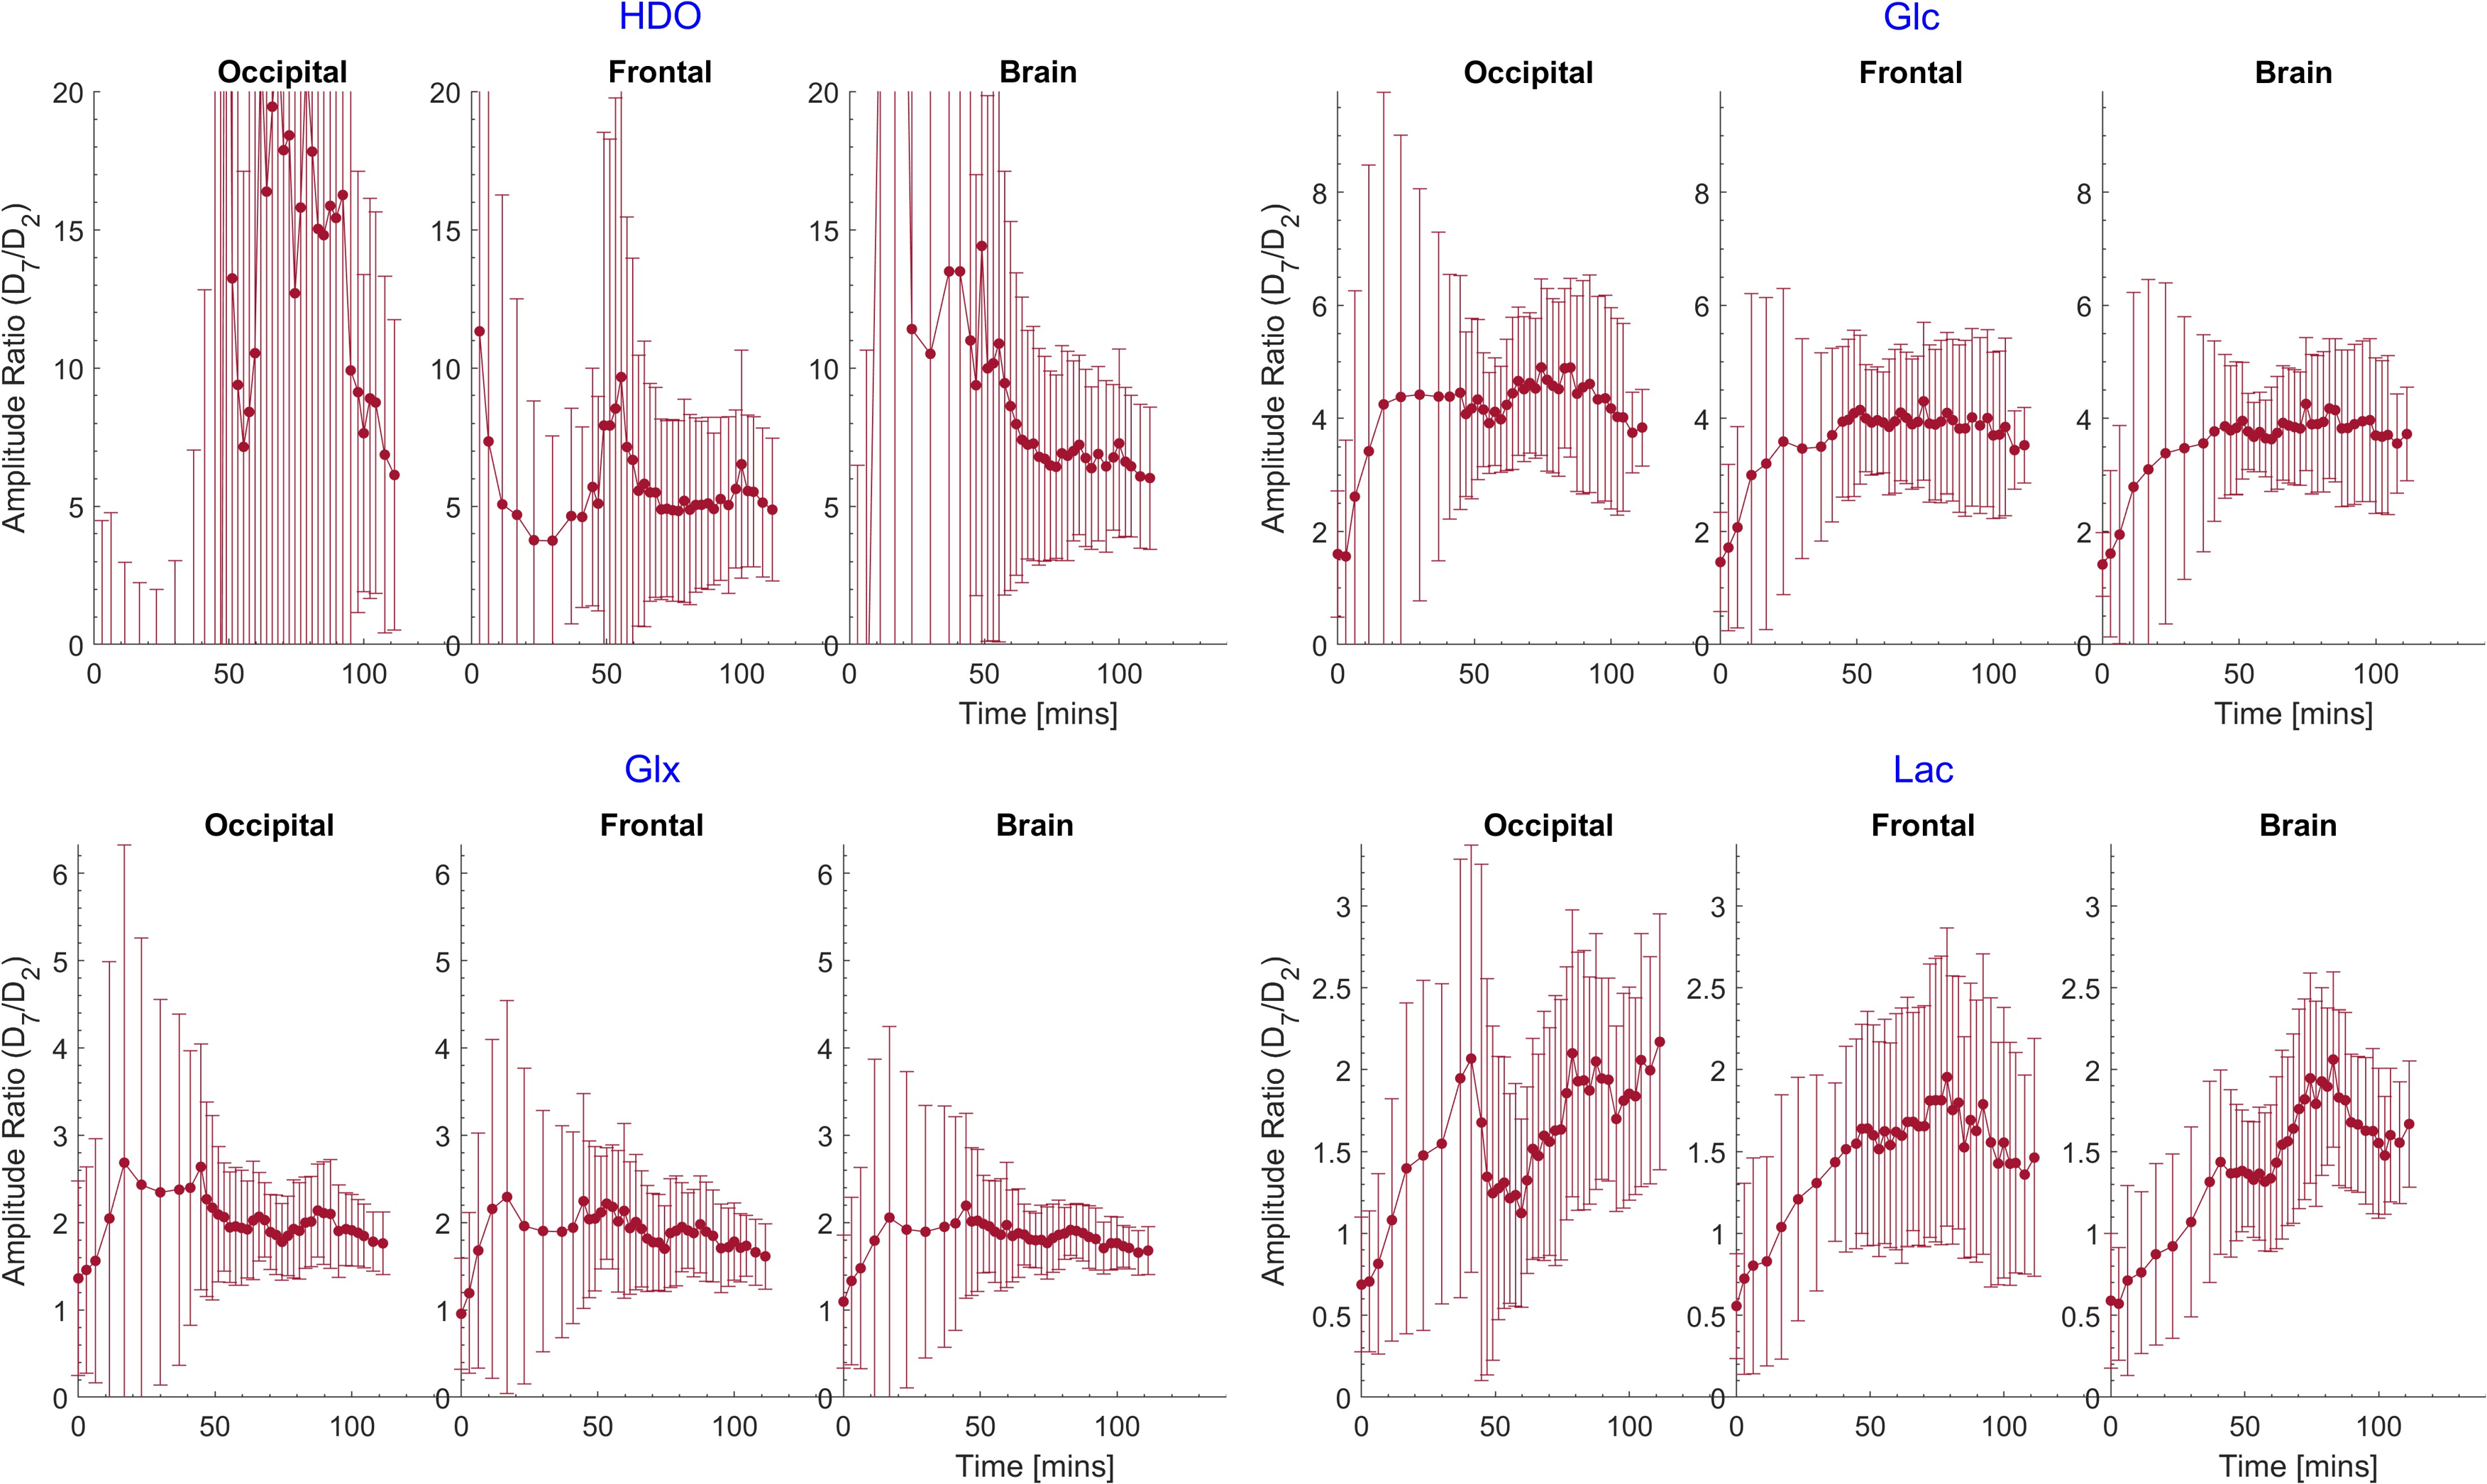
\includegraphics[width = 1\textwidth]{Figures/Glucose/D7_D2.png}
    \caption{Normalised signal intensity ratios for each metabolite of D$_7$- to D$_2$-glucose for the same regions in Figure \ref{fig:Glu:Avg_Conc}. The D$_7$-glucose data is interpolated (after the moving average in Figure \ref{fig:Glu:Avg_Conc}. is applied) to the same time course as the D$_2$-glucose data before the ratio calculation. The amplitude of the errorbars are now the previous standard deviations of the numerator and denominator combined by the standard method of combining independent errors of a quotient.}
    \label{fig:Glu:D7_D2}
\end{figure}

In the plots for HDO, the natural abundance values have been subtracted to produce a ratio of the HDO increases above natural abundance. Although there is considerable variability, focussing on the whole-brain ROI (which should possess the best SNR), it appears that the ratios might be converging to approximately constant values, such that for HDO, glucose, Glx, and lactate, the ratios are 5.5 ± 2.5, 3.5 ± 1.0, 1.6 ± 0.4, and 1.5 ± 0.4, respectively. It has been shown that HDO production from the metabolism of D$_7$-glucose can be used as a biomarker\cite{Mahar2021DeuteratedGlucose}, and showed that the ratio $\Delta$HDO/(Glx+Lac) of T$_1$-corrected signal amplitudes (where $\Delta$HDO is the increase in labelled water above natural abundance) has a quasi-stable value of 2.5, calculated by taking account of label-loss from Glx and lactate, and label-gain to HDO. This ratio is shown in Figure \ref{fig:Glu:HDO_Rat} as well as similar plots for glucose, Glx, and lactate, for both D$_2$ and D$_7$-glucose. The plots of $\Delta$HDO/(Glx+Lac) for D$_7$-glucose appear to also show a quasi-stable region, although at values $<$2.5. Plots for Glx/(Glx+Lac) appear to show long-time convergence to approximately 0.8 which is similar to what has been shown previuosly\cite{Kaggie2022DeuteriumMetabolism}, for both D$_2$ and D$_7$-glucose. However, Glc/(Glx+Lac) plots show global maxima at approximately 30 – 70 minutes, and appear to occur earlier than the maxima of glucose in the plots of Figures \ref{fig:Glu:Avg_Amp} and \ref{fig:Glu:Avg_Conc}.  

\begin{figure}
    \centering
    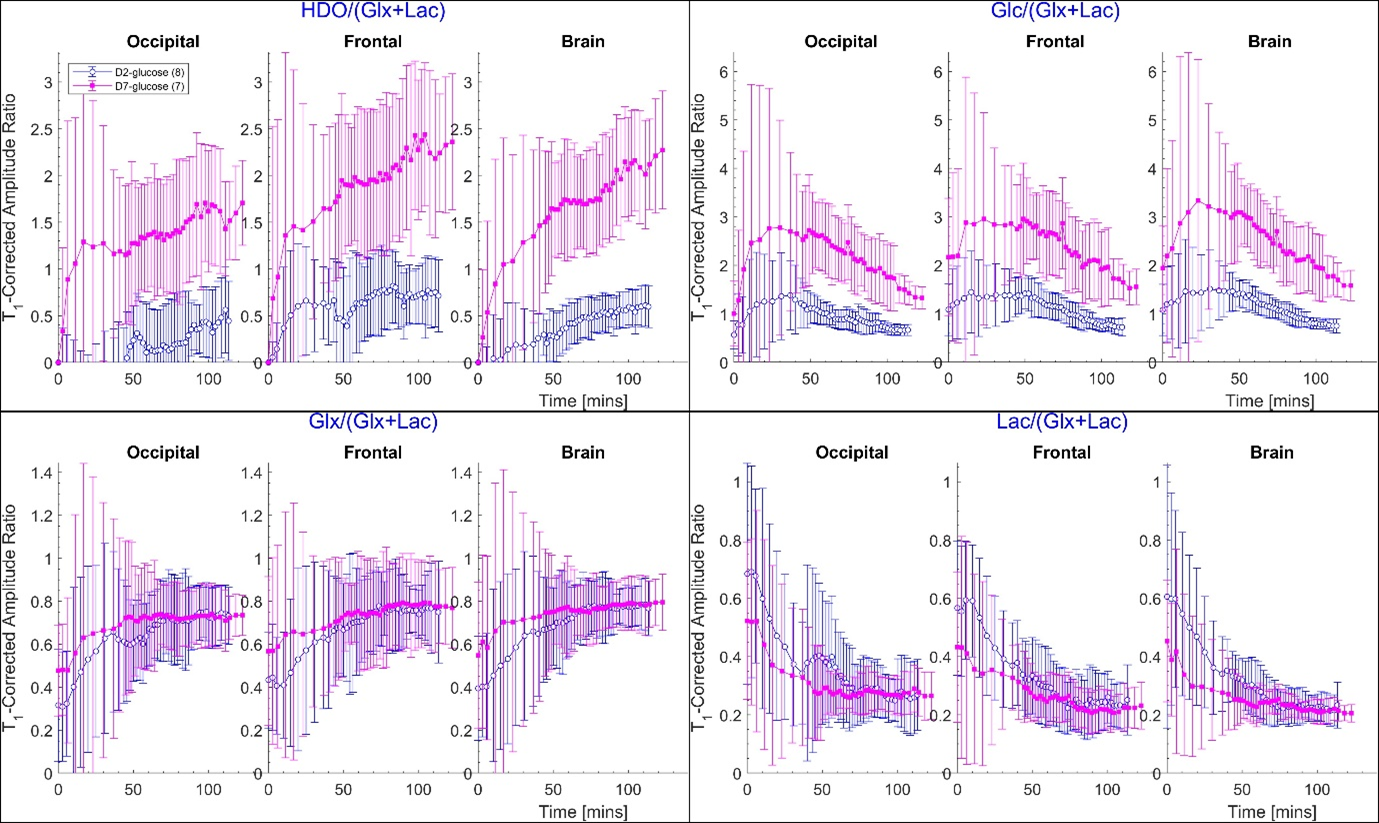
\includegraphics[width = 1\textwidth]{Figures/Glucose/HDO_Ratio.png}
    \caption{Ratio of each metabolite to the sum of downstream metabolites (Glx and lactate) for the same regions in Figure \ref{fig:Glu:Avg_Conc}. The D$_7$-glucose data is interpolated (after the moving average in Figure \ref{fig:Glu:Avg_Conc}. is applied) to the same time course as the D$_2$-glucose data before the ratio calculation. The amplitude of the errorbars are now the previous standard deviations of the HDO amplitude and the denominator combined by the standard method of combining independent errors of a quotient.}
    \label{fig:Glu:HDO_Rat}
\end{figure}

\section{Discussion}

Deuterium spectra and CSI data were acquired from fifteen participants, who had ingested either D$_2$- or D$_7$-glucose, before and at 5 or 6 time points after consumption, with nine of these participants experiencing visual stimulation during the CSI scans. In all spectra, after glucose ingestion, deuterated water (HDO), non-metabolised glucose, and Glx were detected for both glucose isotopologues. Lactate was also detected in most spectra but was present in lower concentrations, particularly for D$_2$-glucose, and was generally more challenging to detect, although average time-courses from all participants revealed an unambiguous accumulation of a deuterated substance at the lactate resonance (see Figures \ref{fig:Glu:Avg_Amp} and \ref{fig:Glu:Avg_Conc}). However, no effect of visual stimulation could be discerned, either in comparison to participants who did not undergo visual stimulation or in comparing metabolite accumulations between frontal and occipital lobes.

 Compared to the CSI data, slice-selective deuterium spectra are quick to acquire and the higher SNR can provide a more reliable analysis if the magnetic field homogeneity is adequate. Such spectra are displayed in Figure \ref{fig:Glu:Select}, showing their time evolution from natural abundance to over 100 minutes after glucose ingestion. These spectra show that HDO (4.8 ppm), glucose (approximately 3.8 ppm), and Glx (2.4 ppm) are clearly visible, with amplitudes being generally larger for the spectra of the participant who ingested D$_7$-glucose, especially for the HDO peak. Although possessing a very low SNR, a peak at 1.3 ppm is just visible in some of these spectra and, again, generally appears to be larger in the D$_7$-glucose spectra. The fact that it is larger in the D$_7$-glucose spectra suggests that it is a result of lactate accumulation but could contain a natural abundance lipid component arising from the skull. Examples of spectral fits are shown in Figure \ref{fig:Glu:Select} for the last time-point spectra in the two displayed data sets. Here it shown that spectral components, including the anomeric decomposition of the two glucose isotopologues, fit well with small residuals.

%

By acquiring multiple chemical shift images, it’s possible to track metabolic flux for glucose and downstream metabolites as has been shown in Figures \ref{fig:Glu:Avg_Amp} and \ref{fig:Glu:Avg_Conc}. By averaging the datasets together, we can also obtain stochastic results of difference in metabolic concentrations which have a higher SNR. Kinetic modelling has been used previously in pre-clinical animal studies using DMI to measure metabolic fluxes10,20,27,42. Only recently kinetic modelling been used once in human participants where D$_2$-glucose was ingested orally43 as opposed to intravenous infusion which was performed in animal models. This modelling allows maximum glucose consumption rates and maximum lactate production values to be determined, which can be performed on a voxel-by-voxel basis assuming the SNR of the individual maps is high enough to allow this. Kinetic Modelling has been applied to the signal amplitude time courses in Figures \ref{fig:Glu:Avg_Amp} and \ref{fig:Glu:Avg_Conc} and is show by the fits.

% CSI data can obviously be improved by performing more averages instead of acquiring multiple CSI data sets at different time points. However, the metabolite time-courses are potentially important, for example, in determining when the glucose signal maximises or if metabolic modelling is to be attempted. Nonetheless, we can get an estimate of what might have been obtained if only a single CSI was acquired with a higher number of averages by combining several of the CSI acquisitions into a single data set. \ref{fig:Glu:CSI} shows this for examples of D$_2$ and D$_7$-glucose data where six consecutive post-glucose-ingestion CSI acquisitions are combined. This would approximately correspond to a single acquisition with 36 averages for a total scan duration of 67 minutes, although this duration could be reduced to xx minutes by the full use of acquisition-weighted averaging (Ref 59). The spectra shown, from a single voxel in the averaged CSI, has the same essential features as the slice-selective spectra in Figure 1; clear HDO, glucose, and Glx peaks, with small low-SNR peaks where lactate is expected. In this case, it is less likely that these peaks contain a large lipid contribution, which suggests that if the peaks are not spurious, they are probably mostly from lactate. 

From \ref{fig:Glu:CSI} it is evident that the metabolite signals are hyperintense in the cortex of the brain with the lateral ventricles appearing hypointense. This is consistent with previous works at ultra-high field12,13, previously this has been difficult to show as more advanced multi-channel coils tend to be more sensitive to the peripheral regions of the brain anyway, however we are using a single-channel birdcage coil which is more sensitive in the centre of the brain. To overcome this issue previous work has shown metabolic maps divided by the HDO signal as it was said to be a good estimate of B1 homogeneity, however, it is shown here that this is not the case here as both types of glucose have distinct metabolic fluxes in HDO signal (D$_7$-glucose being much more metabolically active). The resolution of the acquired CSI data is too low to be able to differentiate GM and WM in the cortex after interpolation. The increase in Lactate signal is clear in Figures 2 and 3 and is statistically significant (p-value) and is larger for D$_7$-glucose compared to D$_2$-glucose (p-value). The increase in lactate production in healthy human participants being detectable agrees with previous literature44. However, it is in contrast with what has previously been seen in healthy human participants at 9.4T where no change in the 1.3 ppm peak, therefore the signal was accredited to lipids12. An explanation for the increase in lactate/lipid signal at 1.3 ppm that isn’t lactate production would be that signal from HDO, glucose and glx signals is being accredited to increase in lactate, to limit this the linewidth bounds for lactate and other metabolite were kept small (20/25 Hz) to limit this effect. 

% From \ref{fig:Glu:CSI} it is evident that the metabolite signals are hyperintense in the cortex of the brain with the lateral ventricles appearing hypointense. This is consistent with previous work at ultra-high field12,13.  The resolution of the acquired CSI data is too low to be able to differentiate GM and WM in the cortex after interpolation. 

% ROI-averaged metabolite amplitudes from individual participant data sets were often noisy and their underlying time-dependence could be obscured (see Figure S2 of the supplementary information). This was more often the case for participants who ingested D$_2$-glucose, whose metabolite amplitudes tended to be lower, but was also an issue for lactate for both glucose isotopologues. Averaging the data over all participants, however, as is presented in \ref{fig:Glu:Avg_Amp}, delivered a clearer picture of the temporal accumulation of the deuterated metabolites. The curves for glucose clearly reach a global maximum within the timeframe of the experiments, and HDO, Glx, and lactate, all unambiguously show increasing trends. The increases in HDO and Glx are as expected from many previous studies, but the observation of an increase in lactate is less common, although it has also been previously measured (Refs 12, 50). Ruhm et al. (Ref 12) showed that the apparent lactate curve probably consists of a non-zero lipid component that possibly has a small time-dependence, plus a small lactate component with a larger time-dependence.     


No significant difference in concentration was detected between participants that had visual stimulus applied and those that didn’t. This can be expected as in the literature only significant increase are seen for lactate45, glutamate, and glutathione, with decreases in aspartate, glutamine, and glycine46. Most of these metabolites are not measurable when doing DMI, and the changes I glutamate and glutamine are in opposing directions which means the change in glx would be smaller. The only other change that could have been detected would have been in lactate, however the inter-subject variability is more than the 10\% increase that has been previously reported.

% No significant difference for any metabolite (HDO, Glc, Glx, and Lac) was seen between participants that had a visual stimulus applied and those that did not. One could compare the metabolism in the frontal lobe and the occipital lobe, however there was a notable difference between the regions in participants who didn’t have visual stimulus applied. Because of the time-course that goes from no detectable signal in glucose, Glx and lactate to a detectable signal it is difficult to compare any other changes above the inter-participant variability which can be larger than 10%. However, it is easier to see metabolite changes using other nuclei such as $^{13}$C, $^{31}$P and $^1$H as there is already baseline measurements so changes are easier to detect. Also, even after a long period the lactate signal is still difficult to detect and fit, so any additional changes are difficult to detect.  

One of the reasons for the large inter-subject variability across all subjects is the evident ‘decrease’ between natural abundance and the first two time points in all metabolite concentrations, most evidently in HDO. This is because at early timepoints the metabolism hasn’t had long enough accumulate increased concentrations above the variability between being repositioned in the scanner. The low SNR of the anatomical $^1$H MPRAGE scan that was acquired could also mean that the ROI’s could be better and represent the regions more accurately, this is backed up by the largest ROI of the whole brain suffering from this effect the least. A more sophisticated multi-channel RF coil would help mitigate this problem and lead to better ROI’s.

% One of the reasons for the large inter-participant variability is the evident ‘decrease’ between natural abundance and the first two time points in all metabolite concentrations, most evidently in HDO. This is because at early time points the metabolism has not had long enough to accumulate increased concentrations above the variability between being repositioned in the scanner. The low SNR of the anatomical $^1$H MPRAGE scan that was acquired could also mean that the ROIs could be better defined and represent the regions more accurately, this is backed up by the largest ROI of the whole brain suffering from this effect the least. A more sophisticated multi-channel RF coil would help mitigate this problem and lead to better ROIs.

The differences in the steady-state signal between the D$_7$- and D$_2$-glucose datasets are similar to what has been theorised from animal models31. These values can slightly alter due to hydrogen-deuterium exchange but ultimately remain stable. They can also change due to label loss, which has been measured in rat models and shown to be stable which means it can be accounted for47. The increase in HDO signal that is generated from the label loss has been quantified in D$_7$-glucose approximately five times when compared to D$_2$-glucose. It has already been shown that the increase in HDO for D$_7$-glucose is an appropriate measure for Warburg metabolism, as the glucose consumption is directly correlated HDO production30. However, the ratio between HDO and glx +lactate is much higher in literature than compared to this study, however it is still evident as shown in \ref{fig:Glu:HDO_Rat}. The difference in ratio could come from the difference in infusion techniques, or it could result from differing amount of label loss.

% The differences in the steady-state signal between the D- and D$_2$-glucose datasets are similar to what has been theorised from animal models31. These values can slightly alter due to hydrogen-deuterium exchange but ultimately remain stable. They can also change due to label loss, which has been measured in rat models and shown to be stable which means it can be accounted for52. The increase in HDO signal that is generated from the label loss has been quantified in D$_7$-glucose approximately six times when compared to D$_2$-glucose. It has already been shown that the increase in HDO for D$_7$-glucose is an appropriate measure for Warburg metabolism, as the glucose consumption is directly correlated HDO production30. However, the ratio between HDO and Glx +lactate is much higher in literature (~2.5) than compared to this study (~1.5), however it is still evident as shown in \ref{fig:Glu:HDO_Rat}. The difference in ratio could come from the difference in infusion techniques, or it could result from differing amount of label loss.

This study has shown the first in vivo studies in human participants using D$_7$-glucose to track metabolism in the brain. This has shown that D$_7$-glucose offers an opportunity to improve the visualisation of Warburg metabolism in vivo for patients, by comparing the concentration levels of metabolites after ingestion of D$_2$-glucose. 


\subsection{Limitations}

Apodisation and smoothing techniques have been shown to affect metabolite quantification in MRSI41, which is why it was chosen to not to apodise when analysing the data. Low-rank denoising has been shown to be able to use the similarities in temporal/spatial information to de-noise, better than for single voxel de-noising37,41. Tucker decomposition also known as a higher order single value decomposition (HOSVD) is an extended version of the simpler SVD, which is then followed by a low rank approximation. Here only the largest singular values persist, and the rest are replaced with zeros, therefore when reconstructed the data is similar except only the most prominent features persist. This works as a de-noising method as the noise will be represented as smaller singular values and will hence be removed, only leaving the metabolite peaks. This can be performed in either the frequency or the time domain. 

% Apodisation and smoothing techniques have been shown to affect metabolite quantification in MRSI47, which is why it was chosen to not apodise when analysing the data. Low-rank denoising has been shown to be able to use the similarities in temporal/spatial information to denoise, better than for single voxel denoising43,47. Tucker decomposition also known as a higher order single value decomposition (HOSVD) is an extended version of the simpler SVD, which is then followed by a low rank approximation. Here only the largest singular values persist, and the rest are replaced with zeros, therefore when reconstructed the data is similar except only the most prominent features persist. This works as a de-noising method as the noise will be represented as smaller singular values and will hence be removed, only leaving the metabolite peaks. This can be performed in either the frequency or the time domain. 

With low SNR datasets it can be possible to bias your data using de-noising, one way to overcome this is to simulate your data and apply varying levels of de-noising which can help choose rank reduction. This was performed with our dataset which helped motivate the choice of rank reduction, which is why de-noising was only applied to each CSI and not with a fifth domain of time. It was found that any level of de-noising in this domain smoothed the metabolite change curves, when compared to individual CSI de-noising. To avoid biasing the lactate peak (because of its low SNR) the simulated data had no true lactate peak present, therefore any presence of lactate above the noise floor in the amplitude maps would indicate too much of a rank reduction. It was found that a rank of eight in the spectral domain and ranks below four in the spatial domain were too small. This compared with the values chosen in previous literature is why we chose our conservative values of 64, 6, 6 and 426,27. 

% With low SNR datasets it can be possible to bias your data using de-noising, one way to overcome this is to simulate your data and apply varying levels of de-noising which can help choose rank reduction. This was performed with our dataset which helped motivate the choice of rank reduction, which is why de-noising was only applied to each CSI and not with a fifth domain of time. It was found that any level of de-noising in this domain smoothed the metabolite change curves, when compared to individual CSI de-noising. To avoid biasing the lactate peak (because of its low SNR) the simulated data had no true lactate peak present, therefore any presence of lactate above the noise floor in the amplitude maps would indicate too much of a rank reduction. It was found that a rank of eight in the spectral domain and ranks below four in the spatial domain were too small. This compared with the values chosen in previous literature is why we chose our conservative matrix dimensions of [64, 6, 6, 4], which are similar to26,27. 

One of the obvious difficulties when attempting fit the D$_7$-glucose data is the extra prior knowledge that has been used, with previous studies fitting the glucose data to as a single peak here the glucose signal is fit as a sum of 14 peaks due to the number of label positions for different anomers $\alpha$ and $\beta$. For completeness the D$_2$-glucose data is fit to 4 peaks for the same reasons, the time increased in the fitting routine between the two fitting routines is approximately 3 times for D$_7$-glucose analysis. The increased complexity of the fitting means it is less likely to accurately fit the FID however by narrowing the linewidth constraints and using more accurate initial estimates, as well as lowering the tolerance of the fit (increasing iterations and function evaluations and lowering the function and step tolerance) the fit overlays the data accurately as seen in Figures \ref{fig:Glu:Select} and \ref{fig:Glu:Avg_Amp}. 

% One of the obvious difficulty when attempting fit the D$_7$-glucose data is the extra prior knowledge that has been used, with previous studies fitting the glucose data to as a single peak here the glucose signal is fit as a sum of 14 peaks due to the number of label positions for different anomers. For completeness the D$_2$-glucose data is fit to 4 peaks for the same reasons, the time increased in the fitting routine between the two fitting routines is approximately 3 times for D$_7$-glucose analysis. The increased complexity of the fitting means it is less likely to accurately fit the FID however by narrowing the linewidth constraints and using more accurate initial estimates, as well as lowering the tolerance of the fit (increasing iterations and function evaluations and lowering the function and step tolerance) the fit overlays the data accurately as seen in Figures 1 and 2. 

\section{Conclusion}

\printbibliography % Comment out main doc

\end{document}